\subsection{Installatie}
Het installeren en opstellen van een nieuwe Drupal 7 core is kinderspel. De minimale systeemvereisten voor een installatie van Drupal 7 zijn verwaarloosbaar. De belangrijkste parameter om te controleren is de versie van PHP. Drupal 7 draait op een PHP versie van 5.2.5 of hoger. 
\newline\newline
De installatie gaat enkel via een Wizard installatie. Deze kan gedownload worden op de officiële website van Drupal. Download de laatste versie van de core en pak deze uit op een plaats waar naar kan gelinkt worden via je lokale server.
Maak nu eerst een lege database aan en surf vervolgens via de browser naar het installatiebestand. Dit is de root directory gevolgd door /install.php. De Wizard begeleid je door het volledige installatieproces. Na de standaard installatie en de taal geselecteerd te hebben, wordt de configuratie van de database ingesteld. Kies welke soort database je wil gebruiker, vul de naam, gebruikersnaam en wachtwoord in. Test de connectie. Aangezien we lokaal werken hoeven geen geavanceerde opties worden ingesteld. We gaan verder en zien dat Drupal wordt geïnstalleerd net zoals alle standaard modules.
\newline\newline
Nadat de installatie voltooid is dienen nog enkele parameters te worden ingesteld. De nieuwe site moet nog een naam en e-mail adres meekrijgen. Er moet nog een Admin worden aangemaakt met bijhorende naam en wachtwoord, alsook een tijdszone van de server. Dit zijn allemaal aanpassingen die niet definitief zijn en kunnen later worden bijgesteld.
\newline\newline
We kunnen nu onze nieuwe Drupal site bezoeken en beheren. De nieuwe site bevat een aantal standaard elementen opgemaakt met een default thema.
\newline\newline
De installatie neemt hooguit 5 minuten in beslag en geeft geen technische moeilijkheden. De installatietijd kan gestaafd worden aan de hand van volgende screencast \citep{LearnByTheDrop2011Installing7}.

\subsection{Theming}
Drupal is een CMS waarbij de aanpassingen grotendeels in de browser gebeuren. Om die reden heeft Drupal twee verschillende thema's actief. Het eerste thema geeft de look en feel van de site. Het tweede is een administratief thema. Dit thema is enkel voor site beheerders. 
Bij het administratief thema is overzicht en duidelijkheid de grootste troef. Hierbij hoeven geen flashy kleuren gebruikt te worden, maar moet een omgeving te vinden zijn waar de administrator alles terug weet te vinden.
\newline\newline
Een standaard installatie van Drupal krijgt voor beide thema's een default toegewezen. In de meeste gevallen zal je bij deze standaard thema's geen genoegen nemen. Indien je opteert af te stappen van een standaard thema heb je drie opties om deze te vervangen.
\newline\newline
Drupal heeft een grote community die ondertussen een lange tijd bestaat. Het aantal thema's dat zowel te verkrijgen is op de Drupal site,als daarbuiten, is immens. Thema's te verkrijgen op de Drupal site zijn allemaal gratis. Externe sites zoals Templatemonsters.com bieden niet minder dan 450 thema's waarvan het grootste deel echter tegen betaling. Deze thema's zijn ready-to-go en hoeven in de meeste gevallen geen aanpassing. Bij het installeren van een thema is het wel mogelijk een aantal parameters in te stellen afhankelijk van het thema.

\begin{figure}[!ht]
  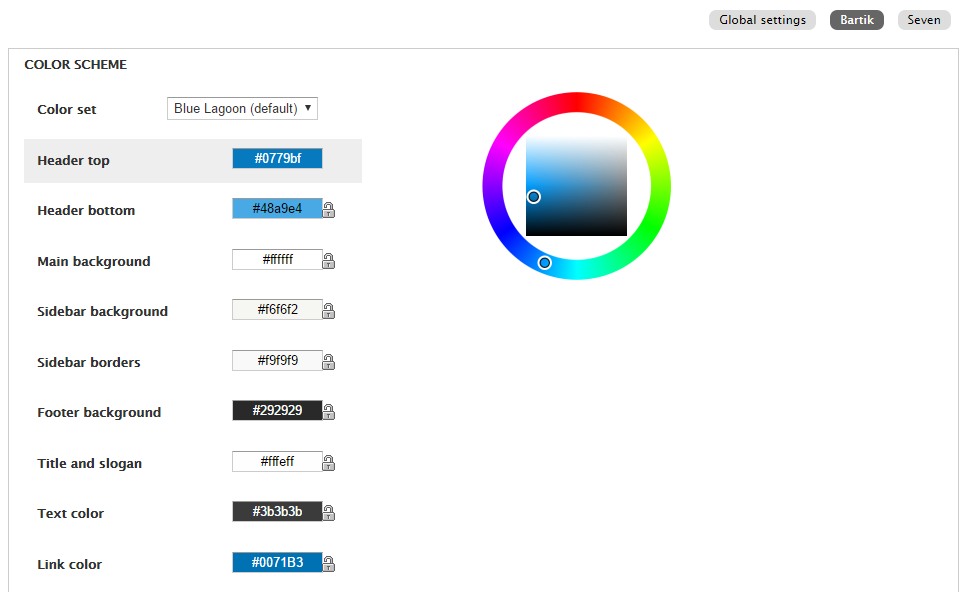
\includegraphics[width=100mm]{img/dr-theme-colors.png}
  \centering
  \caption{Parameters zoals kleuren zijn in te stellen bij sommige thema's.}
  \label{fig:Drupal thema kleuren.}
\end{figure}

\noindent
Een tweede manier van werken is de totaal tegenovergestelde manier. Maak een nieuw thema aan door vanaf nul te beginnen. Maak een folder aan onder volgend pad: projectnaam/sites/all/themes/. Er zijn een aantal stappen en documenten verplicht bij het creëren van een eigen thema. Zorg voor een .info file. Dit document beschrijft je thema. 

\begin{minted}{c}
  name = yourthemename
  description = Description of yourtheme.
  core = 7.x
  engine = phptemplate
  stylesheets[all][] = style.css
  stylesheets[all][] = layout.css
  regions[left] = Left sidebar
  regions[right] = Right sidebar
  regions[content] = Content
  regions[header] = Header
  regions[footer] = Footer
\end{minted}

\noindent
Een thema heeft een naam en beschrijving nodig en draait op een bepaalde Drupal versie. Verder kunnen we CSS files, scripts en regions toevoegen. Regions worden verder in dit hoofdstuk besproken. Via de .info file is het mogelijk het thema te selecteren in de browser. Een site en zeker een thema is niets zonder een opmaak. Daarom voorzie je CSS files in een aparte folder. 
\newline\newline
Van hieraf heb je een thema dat bruikbaar is om mee aan de slag te gaan. Een Drupal thema is gebaseerd op template files die als extensie .tpl.php meekrijgen. Deze files bevatten de html van je thema. Wanneer deze template files niet gedefinieerd zijn in een bepaald thema, worden deze aangesproken vanuit de Drupal core. Wanneer je templates aanmaakt in een thema, overschrijf je met andere woorden de template uit de Drupal core. Templates komen in een aparte folder. In de template page.tpl.php zal je het snelst aanpassingen doen. Deze template bevat de body van de pagina en dus algemene structuur. 

\begin{figure}[!ht]
  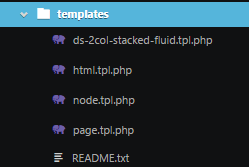
\includegraphics[width=50mm]{img/dr-theme-template.png}
  \centering
  \caption{Template folder van een thema. Overschrijf zoveel template files als nodig.}
  \label{fig:Drupal thema templates.}
\end{figure}

\noindent
Een laatste optie om een thema in te stellen, is een combinatie van de twee voorgaande manieren. Drupal.org heeft een aantal thema's die een basis structuur hebben uitgewerkt. Deze thema's gemaakt met het oog op uitbreiding. Ze bevatten een .info file, een gedeeltelijke of volledige opbouw van een CSS structuur, bijhorende overschreven template files en eventuele andere folders met bijvoorbeeld scripts. Dit soort thema heeft als voordeel dat je niet helemaal opnieuw moet starten maar geeft je een basis om verder op te bouwen. 
\newline\newline
Bij het uitwerken van de casus werd gebruik gemaakt van het basisthema Zen. Dit thema wordt aanzien als populair op Drupal.org. Zen is een eenvoudig HTML5 starters thema met een responsief en mobile-first grid. 
\newline\newline
De opbouw van een pagina loopt gedeeltelijk anders in Drupal in vergelijking met een PHP framework. Zoals reeds aangehaald worden in elk thema regions gedefinieerd in de .info file. Regions bepalen de structuur en gebieden op een pagina. Vaak voorkomende regions zijn een header, footer, een zijbalk, enz. Wanneer de verschillende gebieden zijn aangemaakt kunnen deze worden ingevuld met allerhande content. Regions worden ingevuld met blocks. Blocks zijn aanpasbare blokken die verschillende vormen van inhoud kunnen aannemen. Standaard maakt Drupal enkele block elementen aan zoals menu's, een zoekformulier, shortcuts, enz.

\begin{figure}[!ht]
  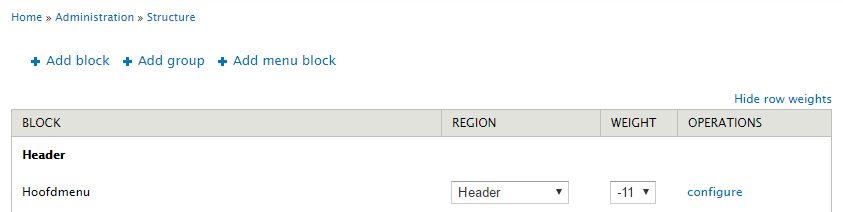
\includegraphics[width=\textwidth]{img/dr-theme-blocks.png}
  \centering
  \caption{Blocks bevatten verschillende bouwstenen van een pagina. Deze zijn terug te vinden onder structuur > blocks.}
  \label{fig:Drupal thema Blocks.}
\end{figure}

\begin{figure}[!ht]
  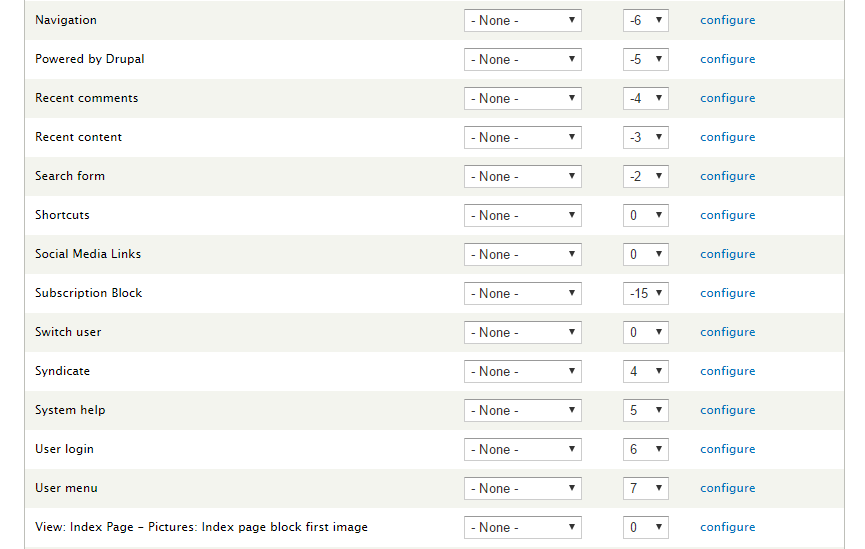
\includegraphics[width=\textwidth]{img/dr-theme-blocks-created.png}
  \caption{Standaard worden reeds enkele blocks voorzien, nieuwe kunnen gecreëerd worden.}
  \label{fig:Drupal thema standaard Blocks.}
\end{figure}

\pagebreak

\subsection{Menu en routing}
\subsubsection{Routing}
Routing in Drupal is een stuk ingewikkelder dan een PHP Framework. Het volledig in detail uitwerken van routing in Drupal valt buiten dit werkstuk. Daarom wordt de algemene werking hier toegelicht.
\newline\newline
Drupal hanteert de database tabel menu\_router om alle verschillende URL's in op te slaan. Wanneer een URL wordt aangevraagd, wordt de volledige tabel overlopen op zoek naar de correcte URL. URL's krijgen steeds een machine naam en alias toegewezen. De machine naam wordt opgeslagen in de database tabel en heeft een weinig zeggende naam voor de gebruiker. De machine naam wordt voorafgegaan door 'node' gevolgd door een cijfer. Een node in Drupal is elk stukje individuele content, zoals een pagina, artikel, blog post, enz. Een alias naam kan per node zelf bepaald worden door de gebruiker. Dit is een haalbare zaak wanneer een site uit een beperkt aantal pagina's bestaat. Indien een site tientallen pagina's bevat is het beter URL's automatisch te laten creëren. De module Pathauto genereert automatische aliassen voor URL's met een beschrijvende naam.

\begin{figure}[!ht]
  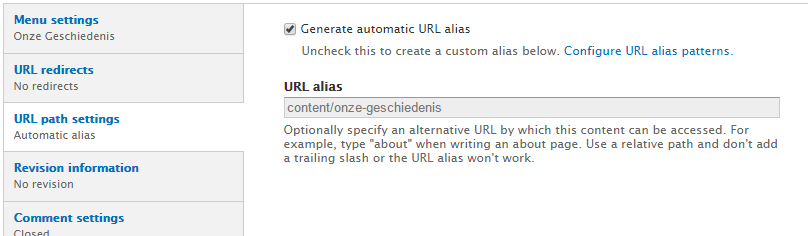
\includegraphics[width=\textwidth]{img/dr-theme-alias.png}
  \centering
  \caption{URL aliassen kunnen automatisch of manueel ingevuld worden per node.}
  \label{fig:Drupal thema alias.}
\end{figure}

\subsection{Menu}
Een menu in Drupal kan volledig beheerd worden via de back-end in de browser. Onder structuur > menu's  worden alle bestaande menu's opgelijst. Standaard maakt Drupal een aantal menu's aan die verder aanpasbaar zijn. Deze menu's zijn eerder gericht op de configuratie van het systeem en van de gebruiker. Links verwijzen naar een gebruikersaccount of naar administratieve taken. Het aanmaken van een menu vraagt weinig kennis. Via de knop 'Add menu' voeg je een menu met een naam en beschrijving toe. Nu kunnen links toegevoegd worden via de 'Add link' knop. Een nieuwe link bevat een naam, pad naar de content en eventuele omschrijving. Dit is de meest eenvoudige opstelling van een menu. 

\begin{figure}[!ht]
  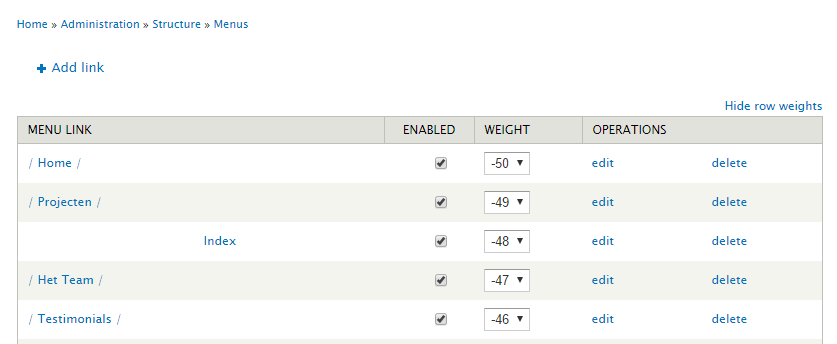
\includegraphics[width=\textwidth]{img/dr-theme-menu.png}
  \centering
  \caption{Aangemaakt menu met bijhorende menu items.}
  \label{fig:Drupal thema menu.}
\end{figure}

\noindent
Een menu kan uitgebreid worden aan de hand van verschillende modules om tot gewenste resultaat te komen. Zo kan een menu bestaan uit submenu's met dropdown functie,  kan een link vervangen worden door een afbeelding of kan een gewicht worden toegekend aan een link. 

\begin{figure}[!ht]
  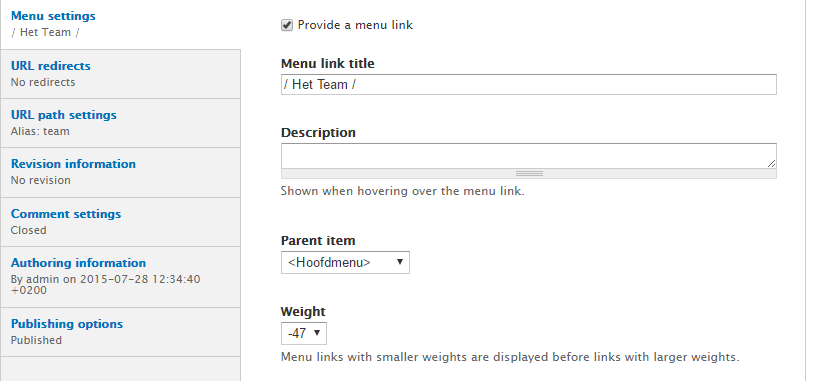
\includegraphics[width=100mm]{img/dr-theme-content-menu.png}
  \centering
  \caption{Wanneer een pagina wordt aangemaakt is het mogelijk direct een menu item te voorzien in een geselecteerd menu.}
  \label{fig:Drupal thema content menu.}
\end{figure}

\pagebreak

\subsection{Plugins en modules}
Drupal 7 gebruikt modules als bouwstenen om sites verder uit te breiden. Drupal is een open source community die een groot aantal gebruikers kent. Elke ontwikkelaar heeft de kans om mee te helpen de community verder te verbeteren en uit te breiden. Meewerken kan door bijvoorbeeld mee te werken aan de core of patches te maken voor modules. Patches zijn verbeteringen aan de code of oplossingen voor bugs. 
\newline\newline
Het aanbod van bestaande modules is immens. Maar liefst 11,894 modules zijn beschikbaar voor Drupal 7 (geraadpleegd op 07/05/2016 \citep{Drupal.org2016DrupalModules}). Modules worden opgedeeld in categorieën, dit zorgt ervoor dat het zoeken naar de gewenste module  eenvoudig en snel verloopt. 
\newline\newline
Installeren van modules is een eenvoudig proces waarbij je op de site van Drupal.org op zoek gaat naar een module. Deze module kan je downloaden als gezipt bestand en uitpakken in de folder project/sites/all/modules. De installatie en activatie van een Module wordt gedaan in de back-end van de browser. Onder de tab modules ga je op zoek naar de nieuwe module en zet je deze op actief. Bij de installatie worden de nodige tabellen aangemaakt en wordt de module gebruiksklaar gemaakt. Afhankelijk van de module kunnen nu de nodige configuratie instellingen gebeuren. 
\newline\newline
Modules kunnen verschillende verhoudingen aannemen. Een module kan een kleine uitbreiding bevatten zoals een extra veld bij content types (content types wordt uitgelicht bij het volgende hoofdstuk). Maar evengoed een uitgebreide module die op zijn beurt nog uitgebreid kan worden met modules. De mogelijkheden met dit soort combinaties is aanzienlijk. In vele gevallen is een grondige kennis van dit soort modules aan te raden. 
\newline\newline
De uitleg, installatie en configuratie omtrent een module is steeds terug te vinden op de bijhorende pagina. Deze uitleg voldoet meestal bij kleine modules, grotere modules voorzien in vele gevallen een eigen tutorial waarbij de deze verder wordt toegelicht.
\newline\newline
Door de hoeveelheid aan modules is de kans dat je voor een bepaald probleem geen oplossing vindt, eerder klein. Toch bestaat de kans dat iets 'custom made' moet gemaakt worden. Het aanmaken van een nieuwe module vergt een grondige kennis van PHP en de werking van de core. De implementatie van een module valt buiten de grenzen van dit stuk. 
\pagebreak

\begin{figure}[!ht]
  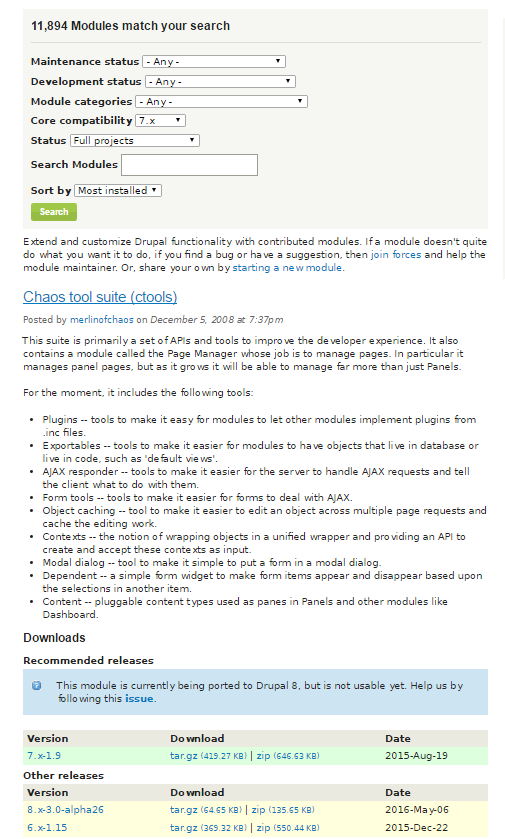
\includegraphics[width=115mm]{img/dr-modules.png}
  \centering
  \caption{Het aanbod aan modules voor Drupal 7 is immens.}
  \label{fig:Drupal modules.}
\end{figure}

\pagebreak
\subsection{Opbouw pagina's}
Dit hoofdstuk beschrijft de werkwijze waarmee de casusopdracht werd verwezenlijkt. Hierin worden  de structuur en het proces in grote lijnen toegelicht.
\newline\newline
Eenmaal de structuur is bepaald via regions kunnen we beginnen nadenken over de verschillende content types. Een content type is een voorgedefinieerde collectie van data types en velden die samen horen. Elke node wordt gelinkt aan een content type. Om de pagina Team te implementeren van de casus, werd een content type aangemaakt. Het aanmaken van het content type teamlid wordt stap voor stap uitgelegd. Via de link structuur > content types kan je een nieuw type aanmaken. Standaard geef je hier de naam en omschrijving mee als parameters. Onder de tab 'Manage Fields' kan je verschillende velden definiëren. Elk veld heeft een label met afgeleide machine naam. Het 'Field type' bepaalt het data type van dit veld. Een Widget is de manier waarop een veld kan worden ingevuld en getoond. 

\begin{figure}[!ht]
  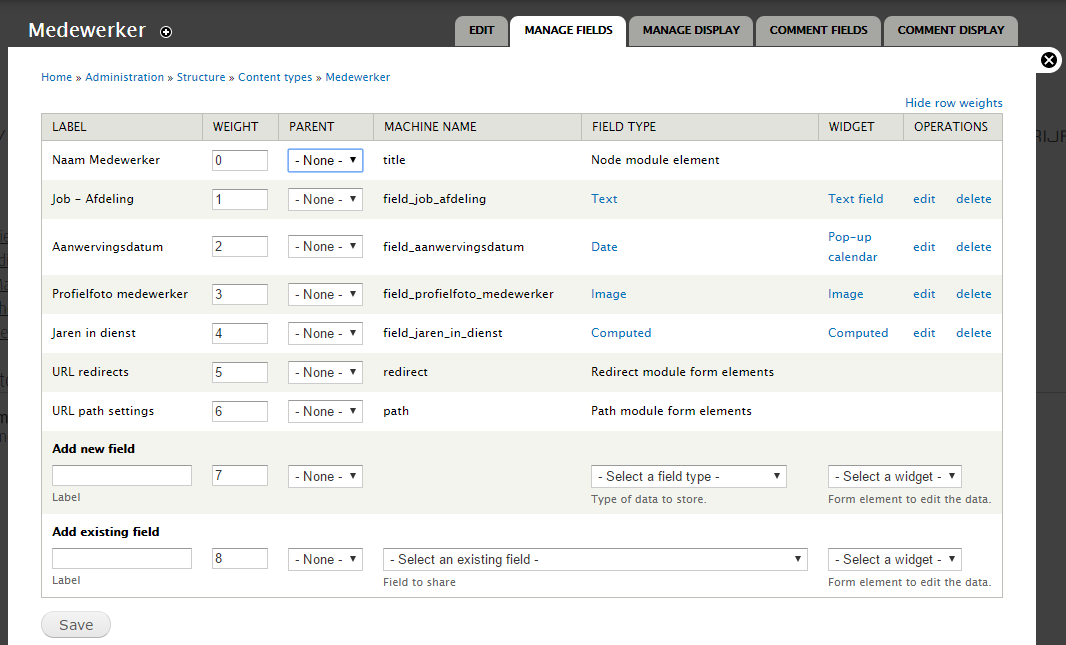
\includegraphics[width=\textwidth]{img/dr-content-type.png}
  \centering
  \caption{Definieer de gewenste velden met bijhorende data types voor iedere content type.}
  \label{fig:Drupal content type.}
\end{figure}

\noindent
De tab 'Manage Display' bepaalt welke velden getoond worden en op welke manier. Velden kunnen al dan niet een label bevatten om het veld te duiden. Een format bepaalt de manier waarop de inhoud getoond wordt. Deze parameters zijn verschillend afhankelijk van het datatype. 
\newline\newline
Standaard kan je kiezen uit een aantal data types. Voldoen deze niet, bestaan er verschillende modules om de data types uit te breiden. 
\newline\newline
Nu het content type voor teamlid is aangemaakt kunnen er leden worden toegevoegd. Een lid kan worden toegevoegd via content > add content > Teamlid. Vul de velden in die eerder werden gedefinieerd in de configuratie van het content type. Bepaal manueel een URL of laat deze automatisch genereren. 
\newline\newline
Alle nieuwe teamleden kunnen bekeken worden in een overzicht via de content link. De volgende stap is het visualiseren van de verschillende leden op een aparte pagina. De leden moeten in een grid van drie kolommen komen te staan. De views module is een zeer uitgebreide module die perfect dienst doet bij problemen zoals deze. Views kan voor vele doeleinden gebruikt worden. Voorstellen van content in een specifieke lijst is één van de meest gebruikte. Elke lijst kan getoond worden als block of als aparte pagina. 

\begin{figure}[!ht]
  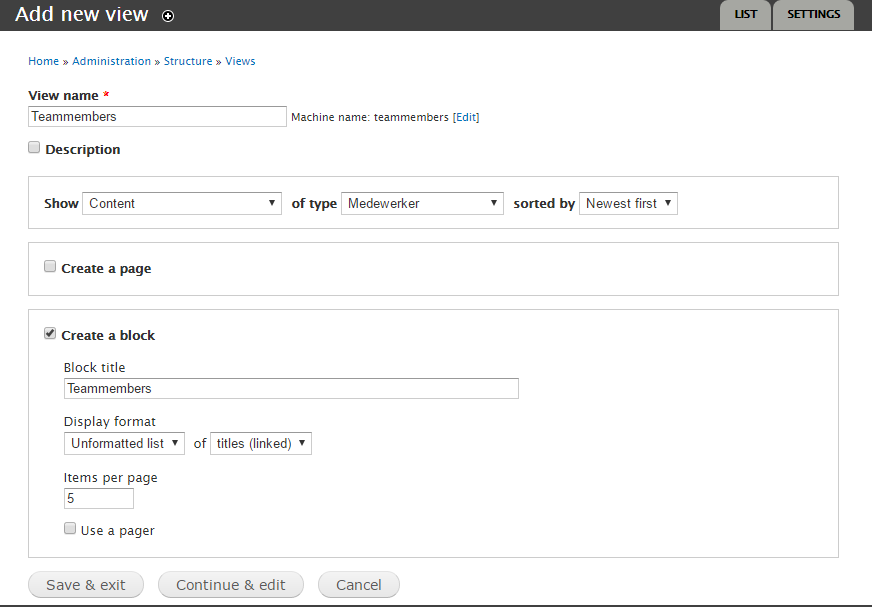
\includegraphics[width=\textwidth]{img/dr-views-new.png}
  \centering
  \caption{Instellingen bij het aanmaken van een nieuwe view.}
  \label{fig:Drupal aanmaken View.}
\end{figure}

\pagebreak\noindent
De view wordt aangemaakt en zal bestaan uit content met als content type Teamlid, aflopend gesorteerd. We zullen de lijst tonen als een block. Later wordt duidelijk waarom. Alle andere instellingen laten we default staan. Alle instellingen die nu gedaan zijn, kunnen achteraf nog aangepast worden. De configuratiemogelijkheden van views zijn oneindig. Daarom is het niet slecht eerst een reeks tutorials te volgen om de belangrijkste opties te leren kennen. Hoewel de meeste opties grotendeels voor zichzelf spreken, kunnen instellingen onder de 'Advanced' tab een view zeer gecompliceerd maken.
\newline\newline
De formattering van de lijst zal gebeuren in een horizontaal grid met drie kolommen. We kiezen ervoor om velden apart te selecteren en in te stellen. Elk gekozen veld kan uitgebreid geconfigureerd worden. Een veld kan bepaalde stijlinstellingen bevatten of herschreven worden.

\begin{figure}[!ht]
  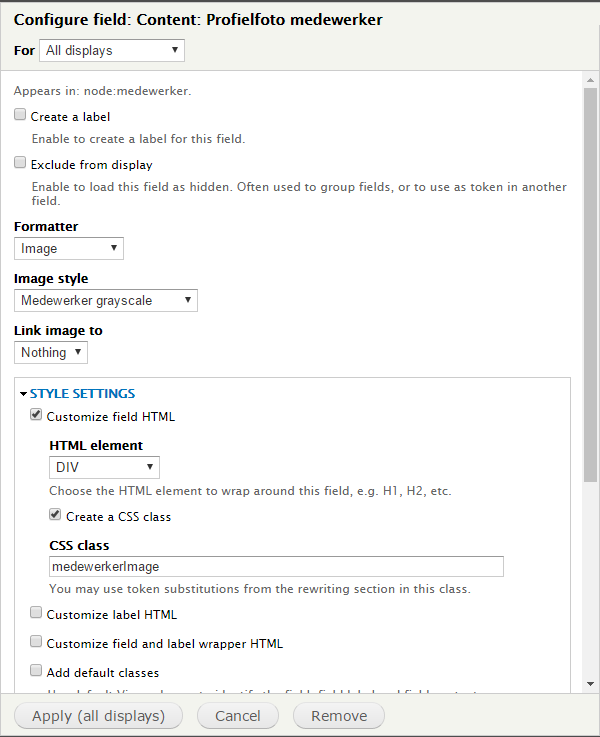
\includegraphics[width=100mm]{img/dr-views-field-setting.png}
  \centering
  \caption{Configuratie van een veld in views Team.}
  \label{fig:Drupal views veld configuratie.}
\end{figure}

\noindent
Inhoud kan een eenvoudige of een gecombineerde filtering bevatten die gesorteerd kan worden op elk type veld. Onderaan wordt een preview gemaakt van de opgehaalde inhoud en hoe deze zich gaat gedragen.

\begin{figure}[!ht]
  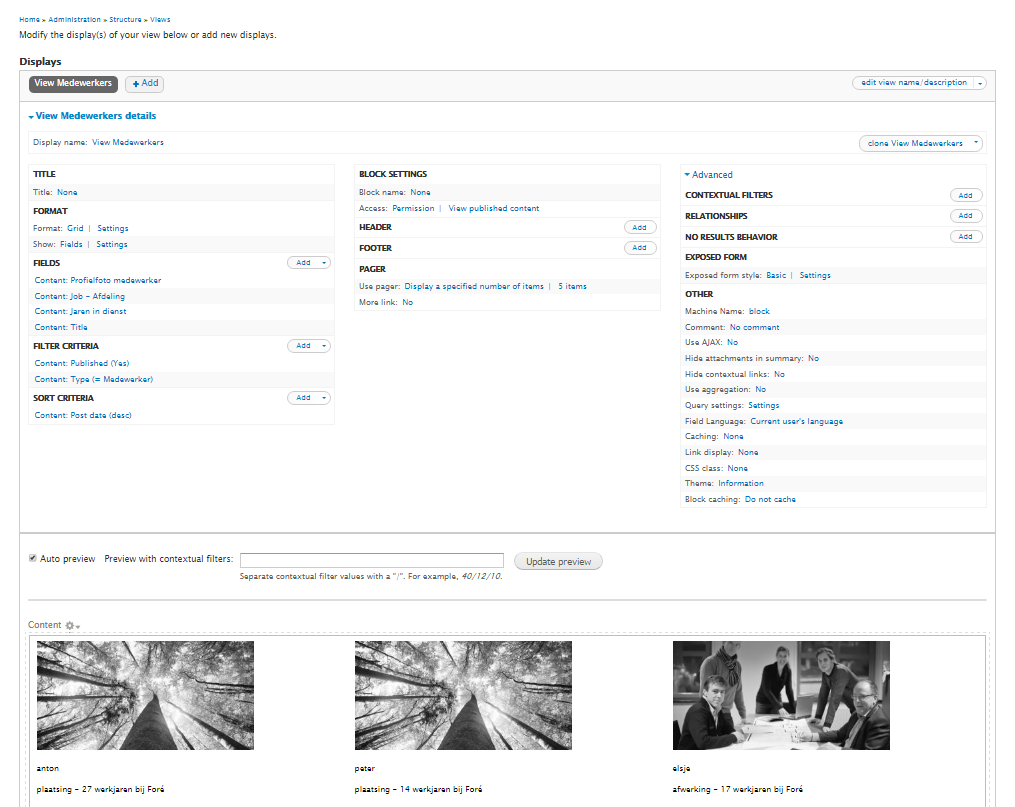
\includegraphics[width=\textwidth]{img/dr-views-team.png}
  \centering
  \caption{Overzicht van de view Team}
  \label{fig:Drupal views overzicht configuratie.}
\end{figure}

\noindent
De view is aangemaakt en staat klaar in een block om getoond te worden op een pagina. Volgens het ontwerp bestaat de pagina naast een oplijsting van teamleden ook uit een banner met bijhorende afbeelding. Voor de banner maken we een apart content type en volgen het zelfde proces als voor teamleden. Er wordt een content type aangemaakt opdat een banner op verschillende pagina's komt te staan. Om de twee blokken inhoud nu in elkaar te smelten gebruiken we de modules page manager in combinatie met panels. 
\newline\newline
Ook panels is een uitgebreide module waar hier slechts het topje van de ijsberg wordt van gebruikt. Wij gebruiken het om twee views samen te laten komen op één pagina. 
\newline\newline
Op de homepagina werd gebruik gemaakt van een eigen gecreëerde layout. Volgens het ontwerp kan je zien dat de homepagina bestaat uit een grid systeem dat niet alledaags is en geen standaard layout keuze is bij panels. 

\begin{figure}[!ht]
  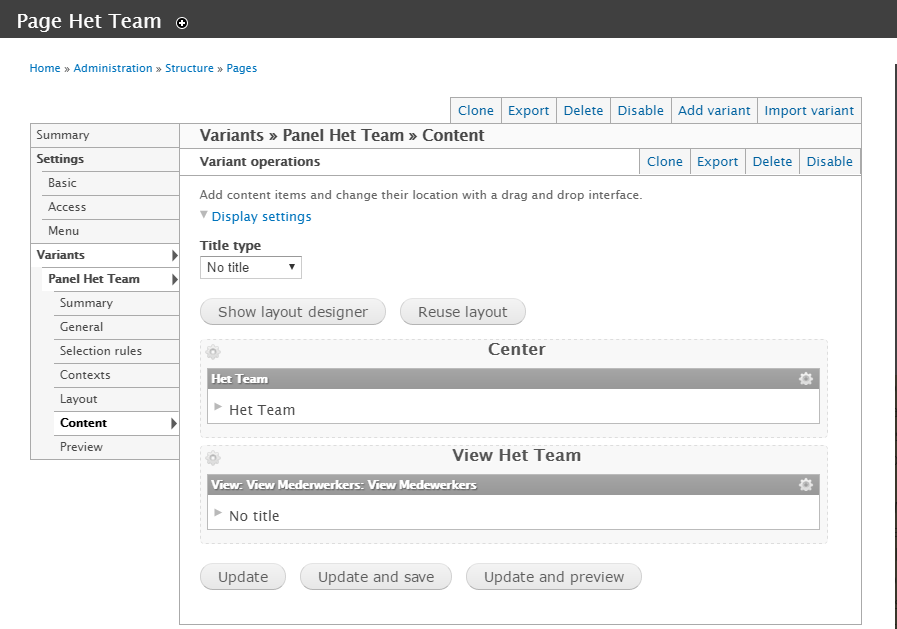
\includegraphics[width=\textwidth]{img/dr-panels.png}
  \centering
  \caption{Team panel pagina, samenvoegen van twee views op één pagina.}
  \label{fig:Drupal page.}
\end{figure}

\pagebreak
